% TODO 20110601
% case        key    value
% annotation  weak   strong
% sharingpool strong weak

% sharingpool:
% HM(V,V)  e.g. string.intern
% a weak hashmap is weak on the keys, so you need to make the values weak, too,
% to avoid a diamond

% versus
% strong key weak value, which is an optimization of the first where the
% canonical object is keyed by some subset of its state

% discussion: weak references let you reference one object, per reference. so
% with a weak map that has $Entry that extend WeakReference, you can reference
% the key XOR the value for free. to reference both weakly references a wrapper

\chapter{Avoiding Memory Leaks by Correlating Lifetimes}
\label{chapter:lifetime-implementation-strategies}

The normal flow of method invocations renders many objects reclaimable, without
any special effort on your part. All temporary objects (see
\autoref{sec:temporary-lifetime}) fall into this camp. These objects are created
and only reachable from local variables of the current method, or of a recent
invocation on the stack. Once these local variables go out of scope, these
temporaries can be reclaimed. A \emph{memory leak} occurs when an object is not
reclaimed in the normal course of method invocations\index{Memory Leak}.
% Typically, objects die soon after the point in time of their last use, once
% all dominating references are removed or naturally go out of scope. In the
% absence of memory leaks, and without any optimizations, objects live and die
% according to this \emph{natural lifetime}, as discussed in depth in
% \autoref{sec:natural-lifetime}.

If you expect an object to be reclaimable at some point, and normal control flow
does not do the right thing, then you need to take a step back and determine how
to properly ensure the lifetime correlation that you expect.
% By relying on objects going out of scope, are insufficient to implement the
% more complicated patterns. Implementations of the correlated lifetime pattern,
% introduced in \autoref{sec:correlated-lifetime-pattern}, are very prone to
% memory leaks.
In some cases, you may need an object to survive for a period of time that is
not bound to any one method invocation, but rather to the lifetime of another
object. In others, the lifetime of an object may actually be correlated with an
invocation, but simultaneously referenced by global variables that inhibit its
timely reclamation. This is a common, and often requisite coding practice.
Oftentimes, the invocation that marks the beginning of a request is in a part of the code
outside of your control, or is distant from the allocation site of the objects
that must go away when the request finishes. In these cases, you should not, or
can not, pass objects around as parameters.

% Implementing a correlated lifetime pattern in a way that does not result in
% memory drag or memory leaks is difficult.
To handle correlated lifetimes in a more robust way requires careful use of some
advanced features of Java. This chapter covers five important cases of
correlated lifetime: annotations, sharing pools, listeners, phase/request-scoped
objects, and external resources.


\section{The (Unachievable) Ideal: The Single Strong Owner Pattern}
% single strong owner is a requirement
% home base is a methodology

A \emph{dominating} (see \autoref{dominance}) reference from object \code{A} to
another \code{B} naturally correlates the lifetime of the two objects. When
\code{A} is reclaimed, then \code{B} becomes reclaimable, because there is no
other way to reach it. This is nice, but requires lining  up many dominoes in
order for things to work as you'd expect. You need to be willing and able to
modify the class definition of \code{A} to add a field, and, what is much more
difficult, you need to ensure that this reference is \emph{the} dominating
reference. Java gives you no way to ensure that the latter is actually the case
--- it's totally up to you, and your careful coding practices. If \code{A} does
not dominate \code{B}, the \code{B} will remain alive, longer than you had
anticipated.

If \code{B} is simultaneously part of multiple data structures, then there's a
good chance that it won't be dominated by \code{A}. The listener pattern,
covered in more detail below, is a common case of this; e.g., the registrar of
listeners for window events becomes a second owner for the window objects. If
so, it becomes hard to keep track of what actions need to be taken in order to
make that object reclaimable by the \jre. From which collections does \code{B}
need to be removed?
% Even if you make your best effort to avoid this problem, such as by using weak
% references, you can still have problems. The diamond structures described in
% \autoref{sec:strongweakdiamonds} are a good example of a case where, even with
% weak references, objects may stick around too long. What programming patterns
% can help to avoid these problems, so that you aren't left hunting down hard to
% diagnose memory leaks late in the development lifecycle?

It would certainly much be simpler if every object were part of only one data
structure at a time.
% This would simplify lifetime management issues, because there would be no
% hidden links for you to track down and eliminate. But, of course, it is often
% necessary for multiple, probably unrelated, parts of the code to need access
% to a common set of objects. : e.g., in user interface code, both the callback
% handler for user events and the redraw loop will operate on the underlying
% data model that the view exposes.
A more relaxed, and achievable, policy would ensure that every object has a 
\emph{home base}. \callout{home-base}{The Home Base as Single Strong Owner}{
% A good design principle is to consider that every object,
If an object simultaneously is part of multiple data structures, then identify
one of these as its \emph{home base}. If possible, you should design for the
home base data structure to be the \emph{single strong owner} of this shared
object. Every other data structure should only weakly reference the object.}

For example, consider an object that is part of a cache. The lifetime policies
of the cache should dictate the lifetime of its entries. When the object is not
in use, the cache is its sole owner, and so this policy is in place.
% If it weren't for the cache holding a non-weak reference to the object, it
% would be reclaimed.
While being used by the program, it may also be part of other data structures.
If these other structures are reachable from non-stack variables, then things
can go wrong. Due to bugs or a developer's oversight, those other data
structures maintain strong references to the object longer than anticipated.
% ; these structures may possibly span multiple threads.
The cache is a natural home base, and any other transient owners of the objects
should be designed so that their ownership is indeed transient: either by being
referenced from the stack, or by being (other than the cache) weakly reachable.

While this design, for practical reasons, is not always feasible, it is
nonetheless something you should keep in mind. Storing strong references to an
object for purposes that are only transient, and forgetting to remove these
references in a timely fashion, is \emph{the} source of memory leaks.
\begin{comment}
A first piece of implementing this single strong owner pattern is the home base
itself:
\begin{shortlisting}
class HomeBase {   
   Set owned = new HashSet();
   
   public void own(Object o) {
      owned.add(o);
   }
}
\end{shortlisting}

%\lstset{moredelim=[is][\underbar]{|}{|}}

On its own, the \class{HomeBase} class provides a repository for strong
references, but doesn't help much in assuring that it is the \emph{only} strong
reference to the objects.To add this extra level of assurance requires four
pieces of logic. First, you need to make sure that every other collection in
which these objects are placed does not have a strong reference to the object.
Second, it would be a big headache to have to call
\class{HomeBase.own()} on every object that you create. This would
heavily pollute your code and be a nightmare to maintain. You can combine the
first two, if there are facades for the collections that take care of the
registration process for you. Third, there are several important use cases for
which the collections are intended to hold data for multiple tasks. Therefore,
you can't simply associate one \class{HomeBase} repository with a
collection; e.g. you may have a single map that contains data for multiple
tasks, each of which needs its own repository. The final issue is how to ensure
that the repository itself becomes reclaimable soon after you are done with it.
A rigorous coding practice is necessary to avoid holding on to the repository
itself for longer than necessary.

You can use a factory design pattern to help. The factory should have this basic
structure:
\begin{shortlisting}
class HomeBaseFactory {
   public HomeBase newOwner() {
      return new HomeBase();
   }

   public Map newMap(HomeBase home) {
      return new WeakHashMap() {
         public Object put(Object key, Object value) {
            home.own(key); return super.put(key, value);
         }
      }
   }
}
\end{shortlisting}
In this base implementation, the \code{newOwner} method doesn't do anything
fancy. But it does provide factory methods for creating a map facade that takes
care of associating ownership with a given repository, while keeping the map
itself free of eternally persistent references to the map's contents. Once the
repository is reclaimed, then the weakly referenced key will be reclaimed, at
which point, or shortly thereafter, the \class{WeakHashMap} will take care of
removing the entire entry (see \autoref{sec:weakhashmap}). From this base
implementation, it should be easy for you to implement similar factory methods
for the other kinds of collections, such as sets and lists.

It is often the case that the repository for ownership can reside within a
thread. If so, you can leverage the \tls mechanism to implement
a factory that provides unique ownership respositories
\begin{shortlisting}
class ThreadLocal_HomeBaseFactory extends HomeBaseFactory {
   ThreadLocal<HomeBase> threadLocals = new ThreadLocal<HomeBase>();
   
   protected void own(Object o) {
      // the thread's HomeBase assumes ownership
      return threadLocals.get().own();
   }

   public HomeBase newOwner() {
      HomeBase home = new HomeBase();
      threadLocals.set(home);
      return home;
      // the caller will now have the only strong reference to the HomeBase repository, we maintain only a weak reference to it
   }
}
\end{shortlisting}

But this implementation suffers from memory drag. After the thread's task
completes, the \tls maintains a reference to the \class{HomeBase} and
all the owned objects. It will only be overwritten either when the same thread is
scheduled to process a new task, or when the thread terminates. You could
overcome this by adding a \code{clear} method, and inserting a call to it at the
right place in your code:
\begin{shortlisting}
public void clear() {
   threadLocals.set(null);
}
\end{shortlisting}
However, this is a messy and error prone solution. An alternative solution is to
rely on local variable scoping to automatically clean things up for you. When a
task begins, you can grab a strong reference to the \class{HomeBase}
repository, and have the \tls maintain only a weak reference to
it:
\begin{shortlisting}
class ThreadLocal_HomeBaseFactory extends HomeBaseFactory {
   ThreadLocal<WeakReference<HomeBase>> threadLocals = new ThreadLocal<WeakReference<HomeBase>>();
      
   protected void own(Object o) {
      // the thread's HomeBase assumes ownership
      return threadLocals.get().get().own();
   }
   
   public HomeBase newOwner() {
      HomeBase home = new HomeBase();
      threadLocals.set(new WeakReference(home));
      return home;
      // the caller has the only strong reference to the HomeBase repository, we maintain only a weak reference to it
   }
}
\end{shortlisting}
Now, all objects owned by the repository will be automatically reclaimable when
the return value of \code{newOwner} goes out of scope.


%Implementations of the time-space tradeoff pattern, introduced in
%\autoref{sec:time-space-tradeoffs-pattern}, can be ineffective if they aren't
%sized properly. They, too, can result in memory exhaustion, e.g. if a cache's
%key misimplement equality, or if it is sized too large.

%It is important to code according to practices that will assure that an object
%dies when it should. The correlated lifetime and time-space tradeoff patterns
%are the most difficult cases to get right, and so those most in need of
%rigorous coding practices.
\end{comment}

\section{Patterns Based on Weak References}
\label{sec:weak-references}
%\autoref{sec:advanced-lifetime-features} introduced the
% advanced features that
%Java provides to help with implementing correlated lifetime patterns in a way
%that avoids memory leaks: finalization, and weak and phantom references. Using
%these features correctly can be difficult. 


As introduced in \autoref{softweak}, Java offers a feature called \emph{weak
references}. Weak references can help you to implement correlated lifetime
patterns in a more flexible way than is possible with normal (strong)
references. They are powerful, but there are ``gotchas'', surprises and
intricasies, that you will need to navigate in order to use them well.
Incautious use of weak references can result in memory leaks that are harder to
debug than the ones you are trying to avoid.

%Normal (strong) references, such as  instance
%and static fields, and local variables, a weak reference provides an alternate
%lifetime implications.

\begin{wrapfigure}[5]{r}{0.44\textwidth}
\centering
\begin{framedlisting}
WeakReference<String> r = new WeakReference("cabbage")
String s = r.get();
\end{framedlisting}
\end{wrapfigure}
A weak reference is manifested as a wrapper object. To weakly reference an
object \code{obj}, you create an instance \code{new WeakReference(obj)}. For the
most part, this weak reference is like any other reference, in the sense that
you can traverse it to access other objects. The only difference is that it does
not inhibit \code{obj} from being reclaimed.
This means that, if \emph{all} paths of references leading to an object contain
at least one weak reference, then
it is an immediate candidate for reclamation. Suc an object is said
to be \emph{weakly reachable}.

To unwrap a weak reference, and retrieve the weakly referenced object, call its
\code{get} method. If this method returns \code{null}, then you know that the
referenced object has been reclaimed. Otherwise, by calling the \code{get}
method on a weak reference, you have now acquired a \emph{strong} reference.

\paragraph{Weak References: Gotchas}
There are many ways to spoil the benefits of weak references. Many of the issues
boil down to having strong references to the weakly referenced object that
inhibit it from becoming reclaimed. When you call \code{get}, you acquire a
strong reference. As long as this strong reference is temporary, say if it is
bound only to the current method invocation, then this new strong reference
shouldn't alter the intended lifetime of the object.   If you were to squirrel
away the resulting strong reference in some other long-lived data structure, you
now have to remember to clip \emph{both} references (this new one, and the
original one that was keeping the object alive up till now), in order to render
the object reclaimable.

%This is a helpful feature, but, on its own, doesn't do
%everything you need in order to implement a correlated lifetime pattern.

\begin{wrapfigure}{r}{0.39\textwidth}
\centering
\begin{framedlisting}
class A {
  WeakReference<B> wrapper;
   
  B getB() {
    B b = wrapper.get();
    if (b != null) {
      return b;
    } else {
      // clean things up
    }
  }
}
\end{framedlisting}
\end{wrapfigure}
You also need to be careful to avoid race conditions. The \code{get} method can
return null at any time, and so you must not expect that a single check for
\code{null} suffices; in-between the first call to \code{get} and the second,
the garbage collector may have, behind the scenes, reclaimed the referenced
object. Instead, call \code{get} once in a basic block, and store the result in
a local variable, as shown on the right.

It gets worse, though. In that code on the right, the \code{else} clause is
intended to do some cleanup in the case that the referenced object is reclaimed.
But the object is gone! The reference is already null, and so you have no way to
pursue any cleaning action. If you need to be informed that the underlying
object has been reclaimed, you must use the \emph{reference queue} mechanism,
introduced in \autoref{sec:reference-queues}.

The standard library, and some third party libraries as well, help with using
weak references correctly. Even then, some care is required.

\paragraph{Weak Maps}
\label{sec:weakhashmap}

\index{WeakHashMap}
The Java standard library includes \class{WeakHashMap}, a class that hides most
of the complexity of managing weak reference queues. This hashmap is a normal
map, excep that it weakly references its keys and strong references its values.
When a key is ready to be reclaimed, the map evicts the corresponding entry.
Behind the scenes, it uses a reference queue, making sure to poll it at the
right times, to know when keys are otherwise reclaimable --- the nice part is
that you needn't worry about any of these details. Your own code is not polluted
by mention of \class{WeakReference} and \class{ReferenceQueue}, nor of the
polling complexities necessary to keep the reference queue from overflowing with
reclaimed keys.

\begin{wrapfigure}[11]{l}{0.36\textwidth}
\centering
\begin{framedlisting}
new MapMaker().concurrencyLevel(8).weakKeys().makeMap();
\end{framedlisting}
\caption{The Guava \code{MapMaker} factory facilitates creating almost any
form of map that you will need. This code creates a concurrent version of the
standard \class{WeakHashMap}.}
\label{fig:mapmaker}
\end{wrapfigure}
\index{Guava, MapMaker}
The Google Guava library~\cite{google-guava} includes a \class{MapMaker} factory
class that provides more general control of the Java advanced referencing
mechanisms. This factory class lets you easily configure whether you want
concurrency or not, whether you need an eviction policy, and whether you need
the keys or values to be specially referenced. The standard Java
\class{WeakHashMap} is not concurrent. You can synchronize it, by using a
\class{Collections.synchronizedMap} wrapper, but it will not be a truly
concurrent map. To make a concurrent analog to the standard \class{WeakHashMap},
you would use the code in \autoref{fig:mapmaker}.

\paragraph{More Weak Reference Gotchas: The Danger of Diamonds}
\label{sec:strongweakdiamonds}

\begin{wrapfigure}[19]{r}{0.42\textwidth}
\centering
\vspace{-5mm}
\begin{framedlisting}
class Key {
  protected void finalize() {
    println("Good");
  }
}
class Value {
  Object key;
}
void add(WeakHashMap map, Value value, boolean diamond) {
  Key key = new Key();
  if (diamond)
    value.key = key;

  map.put(key, value);
}
\end{framedlisting}
\caption{If \code{diamond} is true, then the \code{Good}
message will never appear.}
\end{wrapfigure}
Using a construct such as \class{WeakHashMap} or \class{MapMaker} is not a
guarantee of success. These maps don't control the structure of your keys and
values. A \class{WeakHashMap} weakly references its keys, with the implicit
understanding that the strong owners of the key will properly govern each key's
lifetime. Trouble happens, though, when the value associated with a key strongly
references (possibly indirectly) the key. If you insert values that strongly
reference the key, as illustrated in \autoref{fig:strongweakdiamonds} then the
key will very likely never become weakly reachable, even after the expected
strong reference is reclaimed.

As is shown in the figure, this problematic reference structure has a diamond
shape. The top of the diamond is the \code{Entry} object of the map, from which
emanate two paths to the key, the weak reference from the \code{Entry} to the
key, and the strong reference path that flows through the value. In
\autoref{fig:strongweakdiamonds}, the darkly shaded object has a good chance of
never being reclaimed. 

\begin{figure}   % NMM added [h] just to make formatting look good on 201007023, not necessary
\centering
	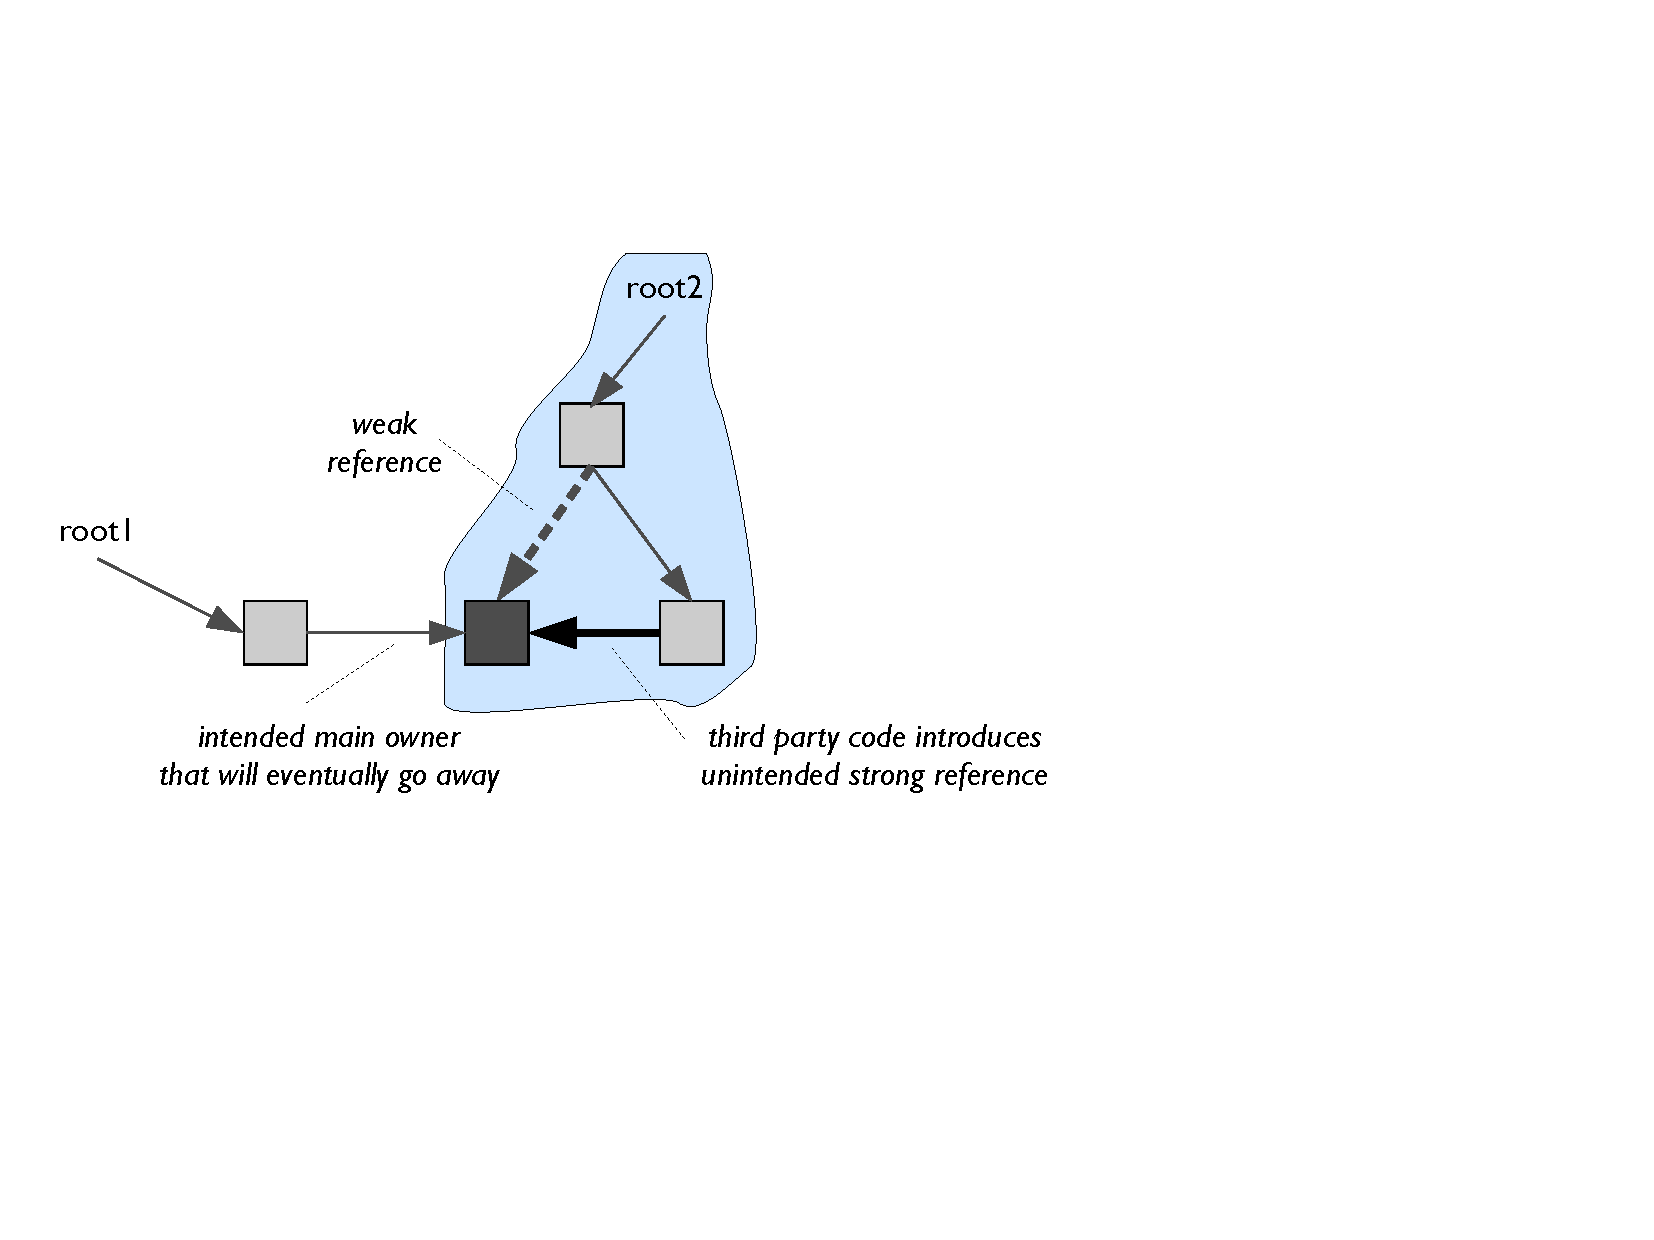
\includegraphics[width=0.6\textwidth]{part2/Figures/lifetime/strongweakdiamonds}
	\caption{Despite your best efforts to use weak references correctly, if you
	introduce a second strong reference in a way that forms a
	\emph{diamond} shape (the shaded region), it will likely never be reclaimed.}
	% [NMM] not sure if we need to give it a name, but, for now
	\label{fig:strongweakdiamonds}
\end{figure}



\subsection{Annotations}

\begin{wrapfigure}{r}{0.43\textwidth}
\centering
\vspace{-3mm}
\begin{framedlisting}
class AnnotationMap<T,A> extends WeakHashMap<T,A> {
  void annotate(T t, A a) {
    super.put(t, a);
  }
}
\end{framedlisting}
\caption{Annotations can make direct use of the \class{WeakHashMap}.}
\label{fig:annotation-map}
\end{wrapfigure}
Normally, to associate information with an object, you would add fields to its
class definition. If you don't have the luxury to change a class definition, but
need to associate some information with it, then your only choice is to use a
side map. The side map is keyed by the object you wish to annotate, and the
value is the annotation itself. Usually, you need the annotation to live no
longer than the annotated object. 

\begin{wrapfigure}[12]{l}{0.4\textwidth}
\centering
\begin{framedlisting}
class TimeAnnotation<T> {
  WeakReference<T> t;
  Date date;
  
  TimeAnnotation(T t) {
    this.t = new WeakReference<T>(t);
    this.date = new Date();
  }
}
\end{framedlisting}
\end{wrapfigure}
To ensure that the lifetime of the annotation is correlated with the lifetime of
the annotated object, you can use a \class{WeakHashMap}. For the most part, you
can use it pretty much in its unadulterated form, as shown in
\autoref{fig:annotation-map}. Soon after an annotated \class{T} instance is
reclaimed, the \class{WeakHashMap} will automatically take care of removing the
annotation entry from the map. If your code updates the annotation map
concurrently with other uses of the map, then you either need to use a
\code{Collections.synchronizedMap} wrapper, from the standard library, or use
the Guava \code{MapMaker} factory (see \autoref{fig:mapmaker}). Even then, you
may suffer some concurrency issues.
\autoref{sec:lifetime-management-concurrency-issues} discusses this issue in
more detail.

You have to be careful to avoid the strong-weak diamond problem described
in \autoref{sec:strongweakdiamonds}.  This is a common and innocent mistake,
because very often it is necessary for the annotations to reference (perhaps
indirectly) the annotated object. This reverse mapping, from annotation to
annotated object, is sometimes necessary to properly implement the annotation's
functionality. Just make sure that the reverse mapping uses a \emph{weak}
reference, otherwise the annotation map will leak memory.
%Careful application of the
%single strong owner principle would help to avoid these mistakes. For example,
%you could offer a factory method 

%\begin{example}{Timestamp Annotation}
%How can you associate a timestamp with an object in a way that avoids memory
%leaks and that scales well to a highly concurrent workload?
%\end{example}
%
%We can start with the following code:
%
%\begin{shortlisting}
%class TimestampAnnotation<T> {
	%T t;
	%long timestamp;
%}
%List annotations;
%for (String string : inputList) {
	%...
	%annotations.add(new WeakReference(new Wrapper<String>(string)));
	%...
%}
%\end{shortlisting}
%
%Despite your use of \class{WeakReference}, you would find that neither the main
%object (the strings), nor the annotations, would ever be collected. This code
%has two memory leaks. One of the leaks is due to a
%violation of the first principal of the use of weak references: the annotations
%strongly reference the objects being annotated. It is not always this easy to
%debug problems in using weak references. Your application will hold on to
%objects that you didn't expect. Quite often, it is difficult to even know that
%there is a problem in the first place! The application may behave normally,
%except that it will consume more memory than necessary; if this extra memory
%consumption pushes it over your maximum heap size, then your application will
%crash --- you will know something is wrong, but diagnosing this type of
%problem, a memory leak\index{Memory Leak}, is quite difficult. It is better to
%keep the three principles of weak references in mind, and design in a way that
%avoids memory leaks in the first place. Your annotations can be modified to use
%a \class{WeakReference} to the main object:
%
%\begin{shortlisting}
%class TimestampAnnotation<T> {
	%WeakReference<T> t; // annotation only weakly refs main object
	%long timestamp;
%	
	%TimestampAnnotation(T t) {
		%this.t = new WeakReference(t);
	%}
%}
%\end{shortlisting}
%
%In this case, the annotation has no normal references to the annotated object,
%and so it obides by the first rule of weak references. If you remember from
%\autoref{chapter:delegation}, the code can be improved further to avoid the
%cost of delegation. This version of the annotation class extends
%\class{WeakReference}:
%
%\begin{shortlisting}
%class TimestampAnnotation<T> extends WeakReference<T> {
	%long timestamp;
%	
%	TimestampAnnotation(T t) {
		%super(t);
	%}
%}
%\end{shortlisting}
%
%Unfortunately, both of these updated versions h?
%%%%%%%
% old version??
%You could store the annotations in a map that is keyed by the
%original object, say of type \class{T}:
%
%\begin{shortlisting}
%Map<T, Date> timestamps = new HashMap<T, Date>();
%
%void addTimestamp(T t) {
	%timestamps.put(t, new Date());
%}
%Date getTimestamp(T t) {
%	return timestamps.get(t);
%}
%\end{shortlisting}
%
%This solution will function correctly, but suffers from a \emph{memory
%leak}\index{Memory Leak}. As the application runs, it will consume greater
%amounts of Java heap, up until the point when the \jre runs out of heap space
%to allocate any more objects. This solution leaks memory, because the
%\code{timestamps} map introduces a reference to the main objects. When the
%garbage collector scans the heap to see which objects are still alive, the
%references in this map will be among those that keep the objects alive. The
%next chapter discusses these issues in more detail. An improved solution would
%use the \class{WeakHashMap} from the Java standard libraries. By replacing the
%initialization of the \code{timestamps} map, we have the same functionality as
%before, but no memory leak.
%
%\begin{shortlisting}
%Map<T, Date> timestamps = new WeakHashMap<T, Date>();
%\end{shortlisting}
%
%Note that this same situation can hold even if you are able to modify the class
%definition. A common scenario requires annotations on only a subset of all
%instances of a class. In this case, is it not worth paying the memory cost to
%have the ability to annotate every single instance. Therefore, this is another
%case where a solution of side annotations, stored in a \class{WeakHashMap},
%shines.
%%%%%%%%%

\subsection{Registrars and Listeners}

Applications that process asynchronous events need a way to decouple event
generation and event handling. For example, it is nice to separate the event
generators, such as windows that generate mouse click events, from the drawing
canvas that will paint the appropriate elements on the screen. This separation
allows for greater flexibility, in case event handlers come and go as the
application runs, or as features are added to the application. It also keeps the
implementations clean of everything but the essential details of the
communication pipe; this example communication pipeline involves only mouse
click events, with no mention of windows or canvases.

The design pattern behind this is called the Listener pattern. Any
implementation of this pattern requires that event handlers register themselves
with an event source. The implementation must keep a registrar of the subscribed
listeners.

This pattern is elegant, but highly prone to memory leaks. The Java Swing
implementation of \class{JComponent} stores an \class{EventListenerList}
instance, which has an array of strong references to the callback handlers.
Because the registrar maintains \emph{strong} references, this approach requires
that you maintain and debug code that explicitly deregisters the callback hook
from the listener queue.


% forgetting to unsubscribe on exception, or forget to call dispose on a larger
% object (window) or window.dispose forgets to unregister itself

\begin{wrapfigure}{l}{0.3\textwidth}
\centering
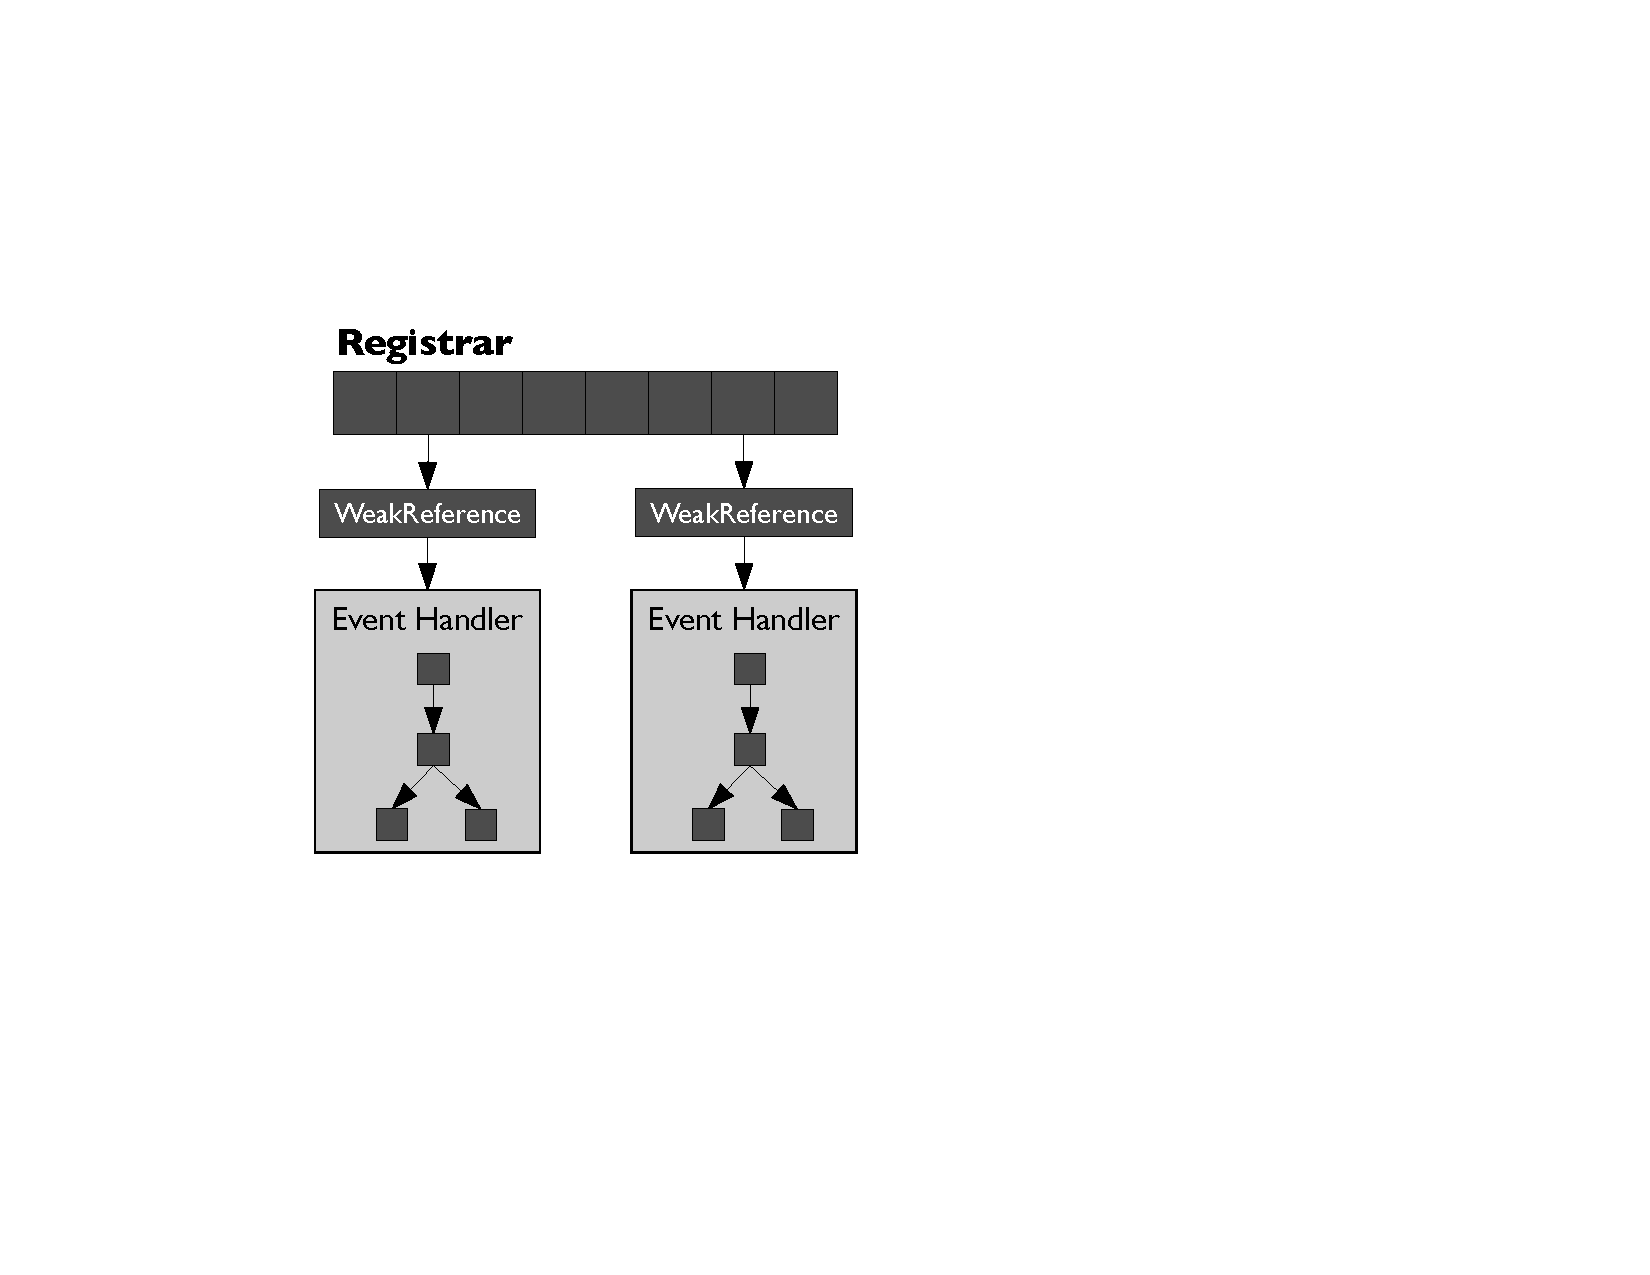
\includegraphics[width=0.3\textwidth]{part2/Figures/correlated/listeners}
\caption{If possible, registrars should weakly reference event handlers.}
\end{wrapfigure}
To avoid this source of bugs altogether, you should consider implementing all
registrars to maintain weak references to the event handlers. With this
referencing structure, there may be no need to explicit deregister event
handlers. Whether or not handlers need to deregister themselves explicit depends
upon the internal structure of the registrar. If the registrar is implemented as
an array-based list, then explicit deregistration is not necessary. When the
handler is reclaimed, the entry in the array will become \code{null}. As long as
you implement the registrar to handle this scenario, everything will work just
fine, without explicit deregistration. If the registar has a more complex,
link-based, structure (such as a \class{LinkedList}), some code must
periodically cull the stale link entries. This is doable, but more difficult
to get right. You may feel safer with explicit deregistration, in this case.

%you must follow the single strong owner principle.
%You must choose which of the listener list or some other collection is the home
%base for the callbacks. For example, if you already have a place to store the
%callbacks, then the listener list can be created by a call to that home base
%factory: {ListenerList list = factory.newList()}.  

\subsection{Sharing Immutable Data Without Exhausting Memory}
\label{sec:sharing-pools-safety}

Storing multiple copies of long-lived data in your heap is wasteful, but
thankfully a relatively straightforward problem to solve.
\autoref{chapter:sharing-immutable-data} introduced the topic of sharing
immutable data. That earlier chapter discussed how to eliminate duplicate data
structures, such as strings, through the use of sharing pools. Pooling the
underlying data allows you store only one canonical copy, and reference it as
needed. The cost of a reference, in Java, will almost always be less than the
cost of duplicating the data in Java objects.

Once you have eliminated duplicate data in your heap, the biggest remaining
concern is that the pools may contain stale data, or even grow in size without
bound. A pool can suffer from memory \emph{drag} (see \autoref{drag} for an
introduction to memory drag) if a pooled data item persists beyond any point in
the code that will use it.

Sharing pools may even suffer from memory leaks (see \autoref{sec:memory-leaks}
for an introduction to memory leaks in Java). In general, if a pool leaks
memory, this is likely to be a sign that your code is misusing the pools. A pool
should contain a bounded number of canonical data items. If it grows without
bound, then either: you were wrong in your assumption that the set of data items
was bounded; or, your lookup mechanism is flawed, and incorrecty indicates that
the pool does not contain a given data item.

In either case, you should protect yourself from the worst effects of memory
drag or memory leaks in your sharing pools. It is pretty easy.

\paragraph{Avoiding Stale Entries in Sharing Pools}


%\paragraph{Example: Annotation Pools}
% For the second requirement, Java provides some support for releasing unused
% items from collections, namely, \class{WeakReference}s and
% \class{WeakHashMap}s. A \class{WeakReference} is an object wrapper. An object
% that is referenced by a \class{WeakReference} can be reclaimed by the garbage
% collector if there are no other strong references to it. A \class{WeakHashMap}
% is a hashmap that stores keys as \class{WeakReferences}. That is, when there
% are no strong references to a key, the entire entry is freed for garbage
% collection.
\autoref{sec:canonicalizing-maps} introduced the canonicalizing map construct. A
canonicalizing map is simply a map from a given instance to the canonical
equivalent (shared) instance. The basic construct is straightforward, but it
takes some care to avoid memory issues. For example, say you are annotating
nodes in a graph. You have an \class{Annotation} for each \class{Node}, and need
the annotation instance to go away when its associated \class{Node}s are no
longer used. This can be implemented by a \class{WeakHashMap<Node, Annotation>}.
Remember that this kind of map weakly references the keys, which means that it
will not, on its own, prevent the node instances from being reclaimed. So, this
looks like all you will need to store the mapping itself. How about storing the
annotations? If every node has its own distinct annotation, then you are done.

If many nodes have the same annotation, then it is worthwhile figuring out how
to share them. If the set of distinct annotations is known statically, then you
can use an enumerated type. If not, then you will need to set up a \emph{second} map, a
canonicalizing map, to maintain the distinct annotations.

The first map, from nodes to annotations, will strongly reference the
annotations. Since you need the annotations to be reclaimed when a node is,
therefore this second map, the annotation canonicalizing map, should only weakly
reference them. This means that the sharing pool of annotations can be
implemented by: \class{WeakHashMap<Annotation, Annotation>}.

This should do it. Wrong! This map suffers from the diamond structure problem
described in \autoref{sec:strongweakdiamonds}. Both the key and the value of
the sharing pool reference the same (canonical) \class{Annotation} object. The
key is a weak reference, but the value is a strong reference, which prevents an
\class{Annotation} object from every being released. The value must also be a
\class{WeakReference}. Here is the correct implementation of a sharing pool for
\class{Annnotation}s:

\begin{figurelisting}
class AnnotationFactory {
   WeakHashMap<Annotation, WeakReference<Annotation>> sharingPool = new WeakHashMap<Annotation, WeakReference<Annotation>>();
    
    public Annotation canonicalize(Annotation annotation) {
        WeakReference<Annotation> wref = sharingPool.get(annotation);
        if (wref != null) {
            Annotation oldAnnotation = wref.get();
            if (oldAnnotation != null) return oldAnnotation;
        }
        sharingPool.put(annotation, new WeakReference(annotation));
        return annotation;
    }
}
\end{figurelisting}

As this example shows,  Java's weak referencing capability has subtle
semantics and is not easy to use.

\paragraph{Avoiding Unbounded Growth in Sharing Pools (Capacity Safety Valves)}
If you already know that your sharing pool has the possibility of growing
without bound, then you should engage the developers to find and fix the
underlying problem. For example, perhaps there truly is not a finite number of
annotations. If, for every new node comes a new annotation, and you have a
steady stream of new nodes, then your sharing pool will leak memory; you will
eventually run out of heap space, and your application will fail.

In some cases, you can protect against this problem. For example, if the map
from node to annotation can be recreated, say from some secondary store, then
you should consider using \emph{soft references}. The node-to-annotation map
should weakly reference the annotations, and the sharing pool
should weakly and softly reference the annotations, as shown in
\autoref{fig:soft-weak-sharing-pool}.

\begin{figure}[h]
\centering
\begin{framedlisting}
WeakHashMap<Node, WeakReference<Annotation>> map;
WeakHashMap<Annotation, SoftReference<Annotation>> sharingPool;
\end{framedlisting}
\caption{A modified form of the sharing pool example that uses soft references
as a safety valve on the maximum memory consumption of the structures.}
\label{fig:soft-weak-sharing-pool}
\end{figure}

In this way, the value of the sharing pool map will be the sole reference
keeping the annotations alive (every other reference is weak). When the \jre
finds that it needs space, that sole non-weak reference will be clipped, thus
starting a cascade that will lead to both weak maps cleaning up the entries. You
will then need to update the node-to-annotation map to detect this case, and
recreate the mapping on demand. \autoref{chapter:trading-space-for-time} goes
into more detail on the use of soft references.


\subsection{Phase/Request-Scoped Objects}

It is a huge challenge to ensure that an object created within a phase or request
dies soon after the phase or request completes. If the object is created at the
top level of the request method, and is never stashed into any static fields or
fields of objects which are bound to enclosing method scopes, then the normal
local variable scoping rules (see \autoref{sec:lifetime-of-locals}) would apply,
and life would be pretty easy:
\begin{shortlisting}
void doLogin() {
   Object obj = new Object();
   restOfWork(obj); // if obj does not escape ...
} // ... then lifetime of obj automatically ends here
\end{shortlisting}
If, during the execution of the \code{restOfWork} method,  \code{obj} does not
escape into some other scope, then its lifetime ends when the \code{doLogin}
method returns; and, possibly, somewhat before that, as discussed in
\autoref{sec:lifetime-of-locals}. The lifetime of the
object \code{obj} will be correlated with the \code{doLogin} request, by the
natural local variable scoping rules. However, it is very easy to write code that
alters the lifetime of \code{obj}. This is especially true if you have a
distributed team that are collaborating to implement the functionality of
\code{restOfWork}. Since the requirement, that the lifetime of \code{obj} be
correlated with the \code{doLogin} request is not specified in the code itself,
and likely not even in comments or documentation, the team does not know to
maintain this lifetime property. For example, a developer may choose to use
\code{obj} as the key into a longer-lived map. This is a common scenario, such
as when \code{obj} is a session identifier that is unique to the user's session
or to the specific request being processed. For example, if you are producing a
page composed of many parts, each part generated by independently written pieces
of code, you can glue them together via a \code{requestState} map:
\begin{shortlisting}
static Map requestState = new HashMap();
void restOfWork(Object requestKey) {
   requestState.put(requestKey, ...);
}
\end{shortlisting}
Now, these instances of \code{obj} will survive for an indefinite period of
time. There is no way to be sure of how long these keys will last, because it
ends on whether any of the \code{obj} intances are equal. If two calls to
\code{restOfWork} are passed equal objects, then the first one will be
reclaimable shortly after its entry in the map is replaced with the new one. 

It is also pretty easy to introduce a memory leak.\index{Memory Leak} If you
stash the object, in this case as a key, into a map, you must plan out a way to
remove it when the \code{doLogin} request is done. One solution is to associate a
cleanup hook with every data structure that should be correlated with a request,
and invoke these at the end of a request. You could use the Listener lifetime
pattern to do this. Each data structure that possibly contains request-scoped
objects must register as a listener. Then, assuming that the request is processed
by a single thread, you could combine the Listener lifetime pattern with a use of
\tls:
\begin{shortlisting}
/* the cleanup API */
interface CleanupHook { ... };

/* every thread keeps a registry of cleanup hooks */
static ThreadLocal<ListenerRegistry<CleanupHook>> requestLocals = new ThreadLocal<ListenerRegistry<CleanupHook>>() {
   public ListenerRegistry<CleanupHook> initialValue() {
      return new ListenerRegistry<CleanupHook>();
   }
}
void doLogin() {
   Object obj = new Object();
   restOfWork(obj); // obj might escape!
   requestLocals.get().notifyAll();
}
\end{shortlisting}

In some cases, this strategy can be made to work. Mostly, though, and even in the
current example, it is not a good approach. The \code{requestState} map is
global, used across all requests. How can you implement a \code{CleanupHook} that
knows which map entries to remove? In general, every data structure in which some
request-scoped objects are stored may have this problem. Each may have a
different requirement for extracting the correct objects, those for the request
that just completed, from the tangle that comes from many other concurrent
requests.

%Also, if your request spans multiple threads, then the above implementation
%simply won't work, because it relies on \tls. Support for
%multiple threads per request that is along the same lines would require
%keepoing track of those threads that participated. It would be pretty
%complicated to get the details working correctly, and maintain them.

How can you design a foolproof strategy that is minimally invasive? It would be
nice to piggyback on the automated reclamation that either local variable
scoping, or weak references offer. A single strong owner factory pattern, where
either a local variable of the top-most method in the request, or \tls, holds the
single strong reference to any request-scoped data:
\begin{shortlisting}
HomeBaseFactory requestLocals = new ThreadLocal_HomeBaseFactory();
void doLogin() {
   HomeBase myLocals = requestLocals.newOwner();
   Object obj = new Object();
   restOfWork(obj);
   // when myLocals goes out of scope, all request scoped objects will automatically become reclaimable
}
static Map requestState = requestLocals.newMap();
void restOfWork(Object requestKey) {
   requestState.put(requestKey, ...);
}
\end{shortlisting}

This implementation avoids the need for you to code any cleanup logic in the maps
and sets that store request-scoped data. You only need to alter the
\emph{constructor} of these maps to use the single strong owner pattern; as long
as you make sure to call \code{requestLocals.set(null)}, then any request-scoped
objects will be reclaimable immediately after the request completes --- all using
the normal, built-in scoping rules. It would be even better if you could arrange
it so that the \class{HomeBaseFactory} is a local variable of the
top-level request method; then, you only need to change the constructors of the
maps and sets that store request-scoped data. There are many minor variations of
this base implementation. You can tailor them to your specific needs.

\section{Patterns Based on Finalization or Phantom References}

\paragraph{Finalization Gotchas}

Behind the scenes,
the \jre allocates an extra object (of type
\class{java.lang.ref.FinalReference}) and stores these in a reference queue
(called the finalization queue). For the most part, these days, the
\class{FinalReference} objects are allocated when the object is queued up for
finalization Some older \jres allocate this object up front, when the object
(that will eventually be queued for finalization) is initially allocated. In
both cases, there is an extra memory overhead associated with using
finalization. Phantom references are a minor variation of finalization that lets
you manage the queues more flexibly: you can use separate queues for different
groups of objects, and manage how often to poll the queues, rather than having a
single queue and relying on the \jre to poll the queue when it feels like
it.\index{References, Phantom}

% 20110525 TODO maybe move to later chapter
Now for the gotchas. First, you can't assume that the finalize method will be
called immediately after the correlated objects death. The Java language
specification does not dictate a timeliness criterion for invoking your
\code{finalize} method. This can lead to dragging of the resources, exactly like
the problem of memory drag described earlier. Second, using finalization
increases memory bloat. For every instance of a class with a \class{finalize}
method, the \jre, behind the scenes, allocates an extra object (of type
\class{java.lang.ref.FinalReference}). This object consumes 28 bytes; the
pointer from the finalization queue adds an extra pointer cost.
\index{Overwhelming the Finalizer Thread}
Third, it is possible to overwhelm the finalization thread. This can happen if
your program creates instances of objects with \code{finalize} methods at a high
rate.
\begin{comment}
 Such is the
case in the following loop:
\begin{shortlisting}
import java.awt.Font;
for (int i = 0; i < N; i++) {
   Font font = new Font("SansSerif", Font.BOLD, 12);
   ... // some small amount of work
   // font does not escape the loop
}
\end{shortlisting}
Since each loop iteration's instance of \code{font} is not used beyond the
execution of that iteration, it seems like one could run this program on a
small heap, for any value of \code{N}. The heap need only fit what it
takes to allocate the handful of objects that represent an instance of
\code{java.awt.Font}. Try it out, for various values of \code{N} and of
\code{-Xmx}! On Sun and IBM \javasix \jres, you will find that, as \code{N}
increases, you will need to increase the maximum heap size allotted to the \jre.
If you don't, this code will fail with a \class{java.lang.OutOfMemoryError}.

The problem, in this case, is that \class{Font} class has a \code{finalize}
method. Therefore, as the loop iterates, instances of \class{Font} begin to pile
up the finalization queue. Periodically, the background finalizer thread wakes
up and cleans up the backlog. But, if this loop nest creates many \class{Font}s
quickly, or there are a large number of threads doing so concurrently, 
the finalizer background thread becomes overwhelmed. Try sticking in this code:
\code{if (i \% 100000 == 0) System.runFinalization()}. Here, you are explicitly
putting your application's thread to sleep in order to let the finalizer thread
catch up. In this case, this change fixes the problem.
\end{comment}


Java provides two other closely related cleanup hooks, in the form of
finalization and phantom references. These hooks are called just after the
garbage collector has discovered that the object is collectible, but before its
memory is reclaimed. If you implement a \code{finalize()} method in a class, then
every instance of that class will go through a finalization process. After being
discovered to be garbage, these instances will be enqueued on a special queue,
usually termed the \emph{finalizer queue}. Most \jres spawn a single thread,
termed the finalizer thread, that periodically scans the finalizer queue,
invoking the \code{finalize} method on the enqueued objects.

Phantom references offer a somewhat more refined version of this pre-reclamation
hook. First, with phantom references, you can associate a cleanup hook on a
per-object basis, rather than, as is the case with finalization, on a per-class
basis. Second, phantom references give you the option of having more than one
cleanup queue and thread, in contrast to finalization where there is a single
finalizer queue and (usually) a single finalizer thread.

You can use the hooks offered by finalization or phantom references to free up
resources that are implicitly associated with an object. Any Java objects
uniquely owned by this object will be reclaimed in the normal course of garbage
collection. It is those resources that are \emph{implicitly} tied to a Java
object, such as file descriptors, socket connections, and database resources such
as compiled queries, that require special attention.

You must be very careful in relying on finalization or phantom references. The
Java language specification provides no assurances of how often, or even whether,
finalization will be run on an object. In the normal course of program execution,
eventually the finalizer will run. This is because the finalizer queue consumes
Java heap, and hence the finalizer thread will always do whatever finalization is
possible before the \jre gives up due to heap exhaustion. However, if your Java
objects serve as proxies for some native, or remote, storage, and the space
consumed by the Java proxies is small compared to the external state, then you
may have problems. The \jre knows nothing about this external state, and so will
not schedule the finalizer thread if an external resource is exhausted.

Furthermore, the specification is very lax about whether finalizers will be run
before program termination. You can ask the \jre to attempt to finalize objects
before the program terminates, by calling
\code{System.runFinalizersOnExit(true)}, a deprecated part of the API. However,
most \jres these days run only a partial finalization, if you ask. It is hard for
the \jre to do the right thing in a deadlock free manner. Should it only schedule
the finalizer thread, which would run any pending finalization? This would be
safe, and is what the \jre will do if you ask. But this misses all the
currently-live objects that would have have been finalized, had the program
reached a point where they were reclaimable. The \jre can't unwind, on exit, all
the Java references thta keep those objects alive. Also, there is no analogous
request to have the \jre run a garbage collection on exit. Hence, even for those
objects which are actually ready to be finalized, the \jre won't do so on exit.
It is for these reasons that the API has been deprecated.

Given these downsides, it is best for you to implement a more robust lifetime
management strategy. If you can establish a correlated lifetime pattern, such as
that the external storage should be reclaimed when an event occurs, or when a
method returns, then you should do so.

\subsection{Cleaning Up External Resources}
\label{sec:external-resources-details}

\subsection{Safety Valves}


\section{Summary}

\begin{table}
\centering
\begin{tabular}{cc}

\end{tabular}
\end{table}


